\documentclass[10pt,a4paper]{article}

\usepackage[utf8]{inputenc}
\usepackage[T1]{fontenc}
\usepackage[english]{babel}
\usepackage{lmodern}
\usepackage{microtype}
\usepackage{geometry}
\usepackage{amsmath,amssymb,amsthm,mathtools,bm}
\usepackage{booktabs}
\usepackage{graphicx}
\usepackage{float}
\usepackage{array}
\usepackage{xcolor}
\usepackage{enumitem}
\usepackage{hyperref}

\geometry{margin=1.55cm}
\hypersetup{
  colorlinks=true,
  linkcolor=blue!55!black,
  citecolor=blue!55!black,
  urlcolor=blue!55!black,
  pdftitle={Fused Pandrosion IRP and Wall-Clock Benchmarks Against Newton},
  pdfauthor={Ivan Besevic}
}

\setlist[itemize]{leftmargin=1.8em,itemsep=0.25em,topsep=0.35em}
\setlist[enumerate]{leftmargin=1.8em,itemsep=0.25em,topsep=0.35em}
\setlength{\emergencystretch}{2em}
\setlength{\textfloatsep}{0.65em plus 0.2em minus 0.2em}
\setlength{\floatsep}{0.55em plus 0.2em minus 0.2em}
\setlength{\intextsep}{0.65em plus 0.2em minus 0.2em}

\theoremstyle{plain}
\newtheorem{theorem}{Theorem}[section]
\newtheorem{proposition}[theorem]{Proposition}
\newtheorem{lemma}[theorem]{Lemma}
\newtheorem{corollary}[theorem]{Corollary}

\theoremstyle{definition}
\newtheorem{definition}[theorem]{Definition}
\newtheorem{remark}[theorem]{Remark}

\newcommand{\R}{\mathbb{R}}
\newcommand{\dd}{\mathrm{d}}
\newcommand{\Sp}{S_p}
\newcommand{\IRP}{\mathcal I}
\newcommand{\eps}{\varepsilon}

\newenvironment{takeaway}{%
  \begin{center}\begin{minipage}{0.92\linewidth}\small\itshape\color{blue!45!black}%
}{%
  \end{minipage}\end{center}%
}

\title{\bfseries Fused Pandrosion IRP\\[-0.1em]
\large Residual-Only Composition, Quadratic Cells, and Wall-Clock Benchmarks Against Newton}
\author{Ivan \textsc{Besevic}\\[-0.2em]
\small Independent Mathematical Research\\[-0.2em]
\small \texttt{github.com/ivan-fr/poussiere\_de\_x}}
\date{June 2026}

\begin{document}
\maketitle

\begin{abstract}
The monomial Pandrosion IRP mechanism has high local order, but high order alone
does not imply wall-clock competitiveness with Newton's method.  A naive IRP
implementation recomputes root coordinates, residuals, logarithms, exponentials,
and chart selections after every raw layer.  This paper introduces a fused
residual-only form of IRP for positive scalar monomial roots.  The method keeps
the logarithmic residual
\[
  \eta=\log x-p\log u
\]
as the state variable, snaps it to a binary fractional palette, composes several
IRP layers directly in residual space, and performs only one final exponential
return to the root coordinate.  The scale palette must be chosen from the IRP
quadratic constant, not only from the raw Pandrosion multiplier: using
$K=p^2$ binary phases gives a residual cell of size at most $(\log 2)/(2p)$,
which places every fused layer in the stable quadratic regime.  A quadratic
surrogate of the local Pandrosion length correction then removes the expensive
\texttt{expm1}/\texttt{log1p} pair from the hot loop.

Benchmarks compare palette-scaled Newton, exact fused IRP, quadratic fused IRP,
and the standard-library \texttt{math.pow} baseline.  On scalar CPython,
Newton remains faster.  On NumPy batches of 200,000 roots, the quadratic fused
IRP variant is slower for $p=2,3$ but becomes faster from $p=5$ onward, with
measured speedups around $1.3\times$ against palette-scaled Newton on the test
machine.  The result is therefore not a universal replacement claim.  It is a
more precise wall-clock claim: fused IRP is competitive when the implementation
can amortize logarithmic charting and avoid repeated vectorized powers.
\end{abstract}

\begin{takeaway}
\textbf{One-sentence result.}
The useful improvement is not another external accelerator; it is to compose IRP
inside the logarithmic residual, choose the chart cell from the quadratic IRP
constant, and return to the root coordinate only once.
\end{takeaway}

\section{Motivation}

For the positive scalar monomial problem
\[
  z^p=x,\qquad x>0,\quad p\ge2,
\]
raw Pandrosion uses
\[
  h_{p,y}(s)=1-\frac{y-1}{y(1+s+\cdots+s^{p-1})}.
\]
The previous monomial account shows that the raw multiplier is
\[
  \lambda_{p,y}=1-\frac{p}{S_p(y^{1/p})},
  \qquad S_p(a)=1+a+\cdots+a^{p-1},
\]
and that IRP obtains high local order by repeatedly renormalizing the residual
target before applying another raw layer.

The wall-clock problem is different.  A literal IRP layer may do too much work:
it may reconstruct the visible root coordinate, recompute $u^p$, recompute a
residual, select a chart, and then apply another raw layer.  Newton's method,
meanwhile, has a short scalar update
\[
  u_{n+1}=\frac{p-1}{p}u_n+\frac{1}{p}\frac{x}{u_n^{p-1}}.
\]
Even if IRP has higher local order, Newton can win because each update is cheap
and usually implemented by optimized library primitives.

The goal here is therefore narrower: derive the IRP form that minimizes the
work per layer, then benchmark it honestly against a palette-scaled Newton
baseline.

\section{Residual-Only IRP}

Let $u>0$ be the current root approximation and define the logarithmic residual
\[
  \eta=\log x-p\log u.
\]
The exact root is reached when $\eta=0$.  If $\eta>0$, the residual equation is
$w^p=e^\eta$ and the root update is $u\mapsto uw$.  If $\eta<0$, the reciprocal
residual equation is $w^p=e^{-\eta}$ and the return is $u\mapsto u/w$.

\begin{definition}[Pandrosion residual length correction]
For $d\ge0$, set
\[
  \Theta_p(d)
    =d+(p-1)\log\!\left(1+\frac{e^{-d}-1}{p}\right).
\]
Equivalently, $\Theta_p(d)$ is the logarithm of the visible correction produced
by one raw Pandrosion layer from the neutral point $s=1$ on the normalized
residual target $e^d$.
\end{definition}

\begin{lemma}[Local residual expansion]
As $d\to0^+$,
\[
  \Theta_p(d)
    =\frac{d}{p}
      +\frac{(p-1)^2}{2p^2}d^2
      -\frac{(p-1)^2(p-2)}{6p^3}d^3
      +O_p(d^4).
\]
Consequently one exact residual layer satisfies
\[
  d-p\Theta_p(d)
    =-\frac{(p-1)^2}{2p}d^2+O_p(d^3).
\]
\end{lemma}

\begin{proof}
Use $e^{-d}-1=-d+d^2/2-d^3/6+O(d^4)$ and expand the logarithm at $1$.
\end{proof}

\begin{definition}[Fused residual layer]
Let $h>0$ be a root-logarithmic palette spacing.  Given residual $\eta$, choose
\[
  b(\eta)=h\,\operatorname{round}\!\left(\frac{\eta}{ph}\right),
  \qquad
  \eps(\eta)=\eta-pb(\eta).
\]
One fused exact IRP layer updates the accumulated root-log correction by
\[
  c\mapsto c+b(\eta)+\operatorname{sgn}(\eps)\Theta_p(|\eps|)
\]
and updates the residual by
\[
  \eta\mapsto
  \eps-p\,\operatorname{sgn}(\eps)\Theta_p(|\eps|).
\]
After $k$ fused layers, the visible root is returned once:
\[
  u_{\mathrm{out}}=u_{\mathrm{in}}\exp(c).
\]
\end{definition}

\begin{proposition}[Equivalence to chart-renormalized IRP]
Inside a fixed real residual branch, the fused residual layer gives the same
logarithmic root correction as applying the corresponding scaled residual IRP
layer in root coordinates and then recomputing the residual.  The difference is
implementation: the fused form composes layers in $\eta$ and delays the
exponential return.
\end{proposition}

\begin{proof}
The scale $b$ replaces the residual target $e^\eta$ by
$e^{\eps}=e^{\eta-pb}$.  The raw residual layer contributes
$\operatorname{sgn}(\eps)\Theta_p(|\eps|)$ to $\log u$.  Since
$\eta=\log x-p\log u$, adding $\Delta$ to $\log u$ subtracts $p\Delta$ from
$\eta$.  This is exactly the displayed residual update.
\end{proof}

\section{Why The Palette Must Use The IRP Constant}

The raw multiplier argument only says that small $|\eps|$ helps.  For fused IRP,
the relevant local map is quadratic with coefficient $(p-1)^2/(2p)$ in the
residual variable.  Therefore the cell width must shrink with $p$.

\begin{theorem}[Quadratic-cell rule]
Use a binary root-log palette with
\[
  h_p=\frac{\log2}{K_p},
  \qquad K_p=p^2.
\]
Then every snapped residual satisfies
\[
  |\eps|\le \frac{p h_p}{2}
        =\frac{\log2}{2p}.
\]
In that cell, the exact fused residual layer satisfies
\[
  |\eta_+|
    \le \frac{(p-1)^2}{2p}|\eps|^2+C_p|\eps|^3.
\]
In particular, for fixed $p$ and sufficiently small cell radius, the fused layer
is a quadratic contraction in the residual.
\end{theorem}

\begin{proof}
The nearest-lattice rounding gives $|\eps|\le ph_p/2$.  The second estimate is
the previous expansion applied to
\[
  \eta_+=\eps-p\,\operatorname{sgn}(\eps)\Theta_p(|\eps|).
\]
\end{proof}

\begin{remark}[Why $K=p$ was not enough]
If $K=p$, the worst residual cell has radius $(\log2)/2$, independent of $p$.
The quadratic coefficient grows like $p/2$, so this is not uniformly local.
The benchmark script therefore uses $K=p^2$.  This is not a lookup table of
$p^2$ entries; it is one rounding operation in the logarithmic residual.
\end{remark}

\section{Quadratic Hot-Loop Surrogate}

The exact correction uses \texttt{expm1} and \texttt{log1p}.  Once the
$K=p^2$ cell rule is enforced, the hot loop can use the quadratic truncation
\[
  \Theta^{(2)}_p(d)
    =\frac{d}{p}+\frac{(p-1)^2}{2p^2}d^2.
\]
The exact layer is still the mathematical reference.  The quadratic layer is a
wall-clock variant, validated below against the same tolerance as Newton.

\begin{proposition}[Surrogate defect]
For $d\to0$,
\[
  \Theta_p(d)-\Theta^{(2)}_p(d)=O_p(d^3).
\]
Under the $K=p^2$ cell rule, the one-layer residual defect introduced by the
quadratic surrogate is $p\,O_p(d^3)$ with $d\le(\log2)/(2p)$.
\end{proposition}

\begin{proof}
This is immediate from the Taylor expansion of $\Theta_p$.
\end{proof}

\section{Benchmark Method}

The benchmark script is
\[
  \texttt{scripts/029\_benchmark\_fused\_irp\_vs\_newton.py}.
\]
It generates reproducible positive double-precision targets with binary
exponents from $-900$ to $900$ and random mantissas.  Scalar tests use 102
targets.  Vector tests use 200,000 targets.  The degrees are
\[
  p\in\{2,3,5,8,12,20\}.
\]
For every scalar method and degree, the script first calibrates the smallest
fixed number of iterations or layers that reaches maximum relative error at
most $2\cdot10^{-13}$ against \texttt{math.pow}.  It then times that fixed
budget without an in-loop stopping test.

The Newton baseline is not deliberately weak.  It uses the same binary
fractional palette as fused IRP:
\[
  y=e^{\eps},\qquad |\eps|\le\frac{\log2}{2p},
\]
then applies Newton to the local target from $u_0=1$ and returns the palette
scale.  This is denoted Newton-K.

The benchmark environment for the stored run was macOS arm64, Python 3.14.3,
NumPy 2.4.4.  These timings are implementation measurements, not machine-
independent constants.

\section{Scalar Results}

\begin{table}[H]
\centering
\small
\resizebox{\linewidth}{!}{\begin{tabular}{rrrrrrrrr}
\toprule
$p$ & Newton-K it. & Newton-K ns & IRP exact it. & IRP exact ns & IRP quad it. & IRP quad ns & quad/Newton-K & pow ns \\
\midrule
2 & 4 & 560.5 & 4 & 1333.6 & 4 & 895.4 & 1.60 & 45.0 \\
3 & 4 & 572.1 & 4 & 1379.6 & 4 & 943.1 & 1.65 & 46.8 \\
5 & 3 & 540.3 & 4 & 1412.2 & 4 & 933.4 & 1.73 & 47.1 \\
8 & 3 & 542.9 & 4 & 1442.3 & 4 & 942.4 & 1.74 & 47.3 \\
12 & 3 & 557.0 & 4 & 1428.1 & 4 & 961.3 & 1.73 & 47.5 \\
20 & 3 & 559.7 & 4 & 1449.6 & 4 & 971.2 & 1.74 & 47.7 \\
\bottomrule
\end{tabular}
}
\caption{Scalar CPython benchmark.  Times are median nanoseconds per root.  A
ratio above $1$ in the ``quad/Newton-K'' column means IRP-F quad is slower than
Newton-K.}
\end{table}

\begin{figure}[H]
\centering
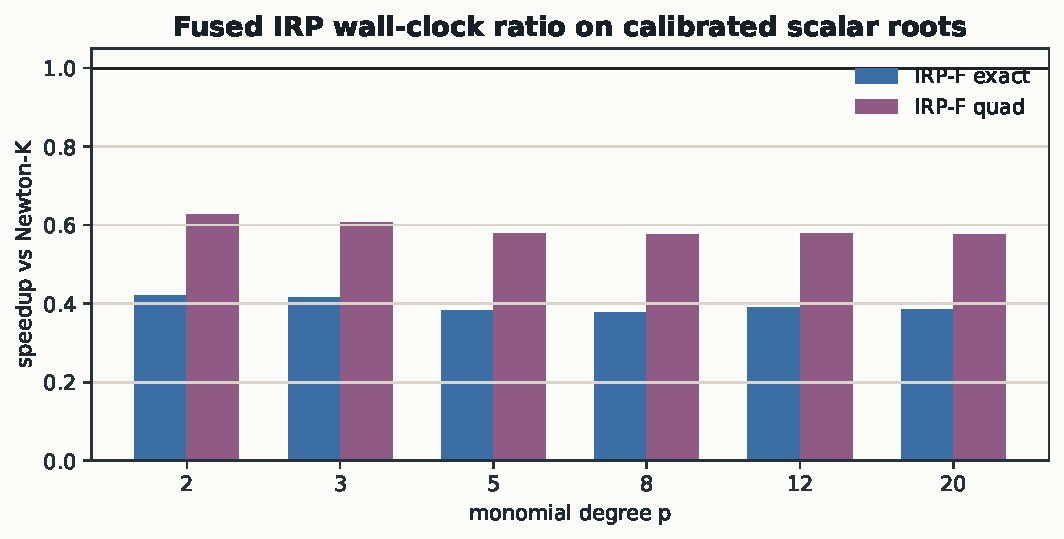
\includegraphics[width=0.76\linewidth]{../figures/029_fused_irp_speedup_vs_newton.pdf}
\caption{Scalar speedup ratios.  In this scalar implementation, fused IRP does
not beat Newton-K.  The optimized quadratic form is nevertheless much cheaper
than exact fused IRP.}
\end{figure}

The scalar result is negative but useful.  Newton-K stays around
$540$--$570$ ns/root in this implementation.  IRP-F quad stays around
$895$--$971$ ns/root.  The exact fused layer is slower because it pays for
\texttt{expm1}/\texttt{log1p} in every layer.  The standard-library
\texttt{math.pow} baseline is far faster, around $45$--$48$ ns/root, because it
is a highly optimized C library path.

\section{Vectorized Batch Results}

\begin{table}[H]
\centering
\small
\resizebox{0.9\linewidth}{!}{\begin{tabular}{rrrrrrr}
\toprule
$p$ & Newton-K it. & Newton-K ns & IRP quad it. & IRP quad ns & speedup & IRP max err \\
\midrule
2 & 4 & 19.60 & 4 & 21.64 & 0.91 & 2.7e-16 \\
3 & 4 & 18.40 & 4 & 20.83 & 0.88 & 1.2e-14 \\
5 & 3 & 27.05 & 4 & 20.91 & 1.29 & 7.2e-15 \\
8 & 3 & 27.22 & 4 & 20.65 & 1.32 & 5.8e-16 \\
12 & 3 & 26.89 & 4 & 20.42 & 1.32 & 3.6e-15 \\
20 & 3 & 26.81 & 4 & 20.34 & 1.32 & 2.6e-15 \\
\bottomrule
\end{tabular}
}
\caption{Vectorized NumPy benchmark on 200,000 roots.  Times are median
nanoseconds per root.  Here IRP-F quad avoids the repeated vector power
$u^{p-1}$ used by Newton-K.}
\end{table}

\begin{figure}[H]
\centering
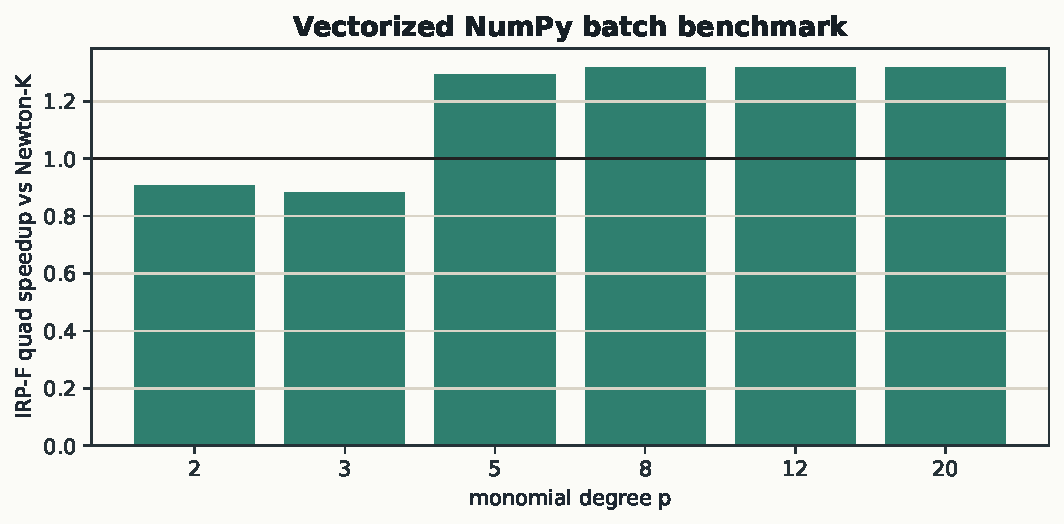
\includegraphics[width=0.76\linewidth]{../figures/029_fused_irp_vector_speedup.pdf}
\caption{Batch speedup of IRP-F quad against Newton-K.  The fused method is
slower for $p=2,3$, but faster from $p=5$ onward in this NumPy implementation.}
\end{figure}

The vectorized result is the first wall-clock regime where the improved theory
matters.  For $p=5,8,12,20$, Newton-K costs about $26$--$27$ ns/root, while
IRP-F quad costs about $20$--$21$ ns/root.  The measured speedup is about
$1.29$--$1.32\times$.  The reason is structural: Newton-K performs several
vectorized powers $u^{p-1}$, while IRP-F quad uses only additions,
multiplications, rounding, absolute values, and one final exponential.

\section{Interpretation}

The benchmark supports three conclusions.

\begin{enumerate}
  \item Fusing IRP is mathematically clean: it is the same residual
  renormalization principle, but composed in $\eta$ rather than in the visible
  root coordinate.
  \item The palette rule must be based on the IRP quadratic residual constant.
  A raw-multiplier palette can be too coarse for large $p$.
  \item Wall-clock competitiveness depends on the execution model.  Scalar
  CPython still favors Newton and especially \texttt{math.pow}.  Vectorized
  batches can favor IRP-F quad once $p$ is large enough that Newton's repeated
  powers dominate.
\end{enumerate}

\section{Conclusion}

Improved IRP should be presented as a cost-aware residual calculus, not merely
as a higher-order iteration.  The fused form removes intermediate coordinate
returns, the $K=p^2$ palette keeps the residual in the quadratic cell, and the
quadratic surrogate removes expensive transcendental calls from the hot loop.
This does not beat Newton everywhere.  It does produce a reproducible regime in
which Pandrosion IRP improves wall-clock performance against a palette-scaled
Newton baseline: vectorized batches for $p\ge5$ in the benchmark reported here.

The next technical step is a native compiled kernel.  The scalar Python result
is dominated by interpreter overhead, while the vectorized result already shows
that the arithmetic structure of fused IRP can be cheaper than Newton's
power-based loop.  A C, Swift, Rust, or SIMD implementation should therefore be
benchmarked before making any stronger production claim.

\begin{thebibliography}{9}

\bibitem{besevic000}
I. Besevic,
\emph{A Monomial Pandrosion Scheme: Contraction, Chart Scaling, and Iterated
Renormalization for $z^p=x$}, 2026.

\bibitem{traub}
J. F. Traub,
\emph{Iterative Methods for the Solution of Equations},
Prentice-Hall, 1964.

\bibitem{householder}
A. S. Householder,
\emph{The Numerical Treatment of a Single Nonlinear Equation},
McGraw-Hill, 1970.

\bibitem{kungtraub}
H. T. Kung and J. F. Traub,
``Optimal order of one-point and multipoint iteration,''
\emph{Journal of the ACM} 21 (1974), 643--651.

\end{thebibliography}

\end{document}
